\documentclass{report}
\renewcommand{\thesection}{\arabic{section}}

\usepackage{titling}
\usepackage{blindtext}
\usepackage{amsmath}
\usepackage{amssymb} 
\usepackage{hyperref}
\usepackage{totpages}
\usepackage{natbib}
\usepackage{float}
\usepackage{afterpage}
\usepackage{algpseudocode}
\usepackage{listings}
\usepackage{graphicx}
\usepackage[titletoc, title]{appendix}
%%%%%%%%%%
\begin{document}

\title{
  CS3263 -- Foundations of Artificial Intelligence
  \\
  Term Project Report
  \\
  \vspace{2cm}
  SmartFridge, an AI agent that recommends the best recipe for you
  \vspace{4cm}
}


\author{
    \textbf{Lei Jianwen} (A0281480E, \texttt{e1155608@u.nus.edu}) \\
    \textbf{Chen Yixun}  (A0281405L, \texttt{e1155533@u.nus.edu}) \\
    \textbf{San Muyun}   (A0271888J, \texttt{e1121291@u.nus.edu}) \\
}

\date{\today}
\maketitle

% Defining new variable terms
\newcommand{\Fridge}{\mathcal{F}}
\newcommand{\RecipeMenu}{\mathcal{M}}
\newcommand{\food}{\mathit{f}}
\newcommand{\recipe}{\mathit{r}}
\newcommand{\days}{\mathit{days}}
\newcommand{\fname}{\mathit{f\_name}}
\newcommand{\fty}{\mathit{fty}} % Food type
\newcommand{\sty}{\mathit{sty}} % Storage type
\newcommand{\FT}{\mathit{FT}} % Set of food types
\newcommand{\ST}{\mathit{ST}} % Set of storage types

% Elements of FoodType
\newcommand{\CANNED}{\text{CANNED}}
\newcommand{\VEGFRUIT}{\text{VEG\_OR\_FRUIT}}
\newcommand{\MEAT}{\text{MEAT}}

% Elements of StorageType
\newcommand{\REFR}{\text{REFRIGERATE}}
\newcommand{\FRZN}{\text{FROZEN}}
\newcommand{\NORM}{\text{NORMAL\_TEMP}}

\section{Introduction}
\subsection{Motivation}
Research has shown that households often waste food because expiration dates are overlooked and meal planning is not done systematically. The amount of avoidable food waste is equivalent to each household throwing away a 2.5kg bag of rice every week. And over half such waste can be reduced if meals are better planned. Recognizing this issue, our team aims to develop an AI-driven solution. An AI-driven menu suggestion system can address this challenge by tracking food items, reasoning about their freshness, and proposing meal options that prioritize ingredients with shorter expiration dates.

\subsection{Project Scope}
Our solution contains the following features
\begin{itemize}
    \item Keep track(Add/Delete) food items from the fridge
    \item Keep track(Add/Delete) recipes from a recipe book
    \item Recommend the most suitable recipe from the recipe book
\end{itemize}

\subsection{Techniques Used}
The recommendation is simulated by a decision-making process to decide which recipe to recommend. A decision tree is constructed to solve this problem. The parameters of the decision tree can be categorized into two types. Two Bayesian networks are implemented to calculate the feasibility of the recipe and probabilities of expiration of food items. The utility function for each recipe is calculated using an unsupervised machine learning model.

\subsection{Terminology \& Notations}

For clarity, the main symbols and assumptions used in this report is defined below:

\begin{itemize}
    \item $\Fridge = \{ \food_1, \food_2, \dots, \food_n\}$ denotes the set of food items available and currently stored in the fridge.
    \item Each food item $f_i$ is associated with food names $\fname_{\food_i}$ days in the fridge $\days_{\food_i}$, food type $\fty_{\food_i}$, storage type $\sty_{\food_i}$.
    \item $\forall \fty_{\food_i}, \fty_{\food_i}\in \FT, \FT = \{ \CANNED, \VEGFRUIT, \MEAT \}$. To simplify the problems, we only focus on these three types of food.
    \item $\forall \sty_{\food_i}, \sty_{\food_i}\in \ST, \ST = \{ \REFR, \FRZN, \NORM \}$. Similarly, we limit the scope of the discussion to only these three types of storage.
    \item $\forall \fname_{\food_i}, \fname_{\food_i} \in \FoodNames$, $\FoodNames$ is the set of food names available in the fridge.
    \item $\RecipeMenu$ is the set of recipes that will be available for users. A fixed set of recipes has been redifined with its relevant attributes.
    \item Each recipe $\recipe_i$ has an unique attribute of recipe name $\recipen_{\recipe_i}$.
    \item Each recipe $\recipe_i$ has a requirements in form of a set of names of the required food items $\requirements_{\recipe_i} = \{ \fname_{F} | \fname_{F} \in \mathcal{N} \}$.
    \item 
\end{itemize}
\section{Bayesian Network Inferencing}
The probability of successfully making the recipe depends on various foods available in the fridge. In order to infer the probability of the success, a Bayesian Network is used for modeling.

\subsection{BN structure}
This can be seen from the picture Figure~\ref{fig:BN}
\subsection{Learning}

\subsection{BN reasoning}
\section{Utility theory}
Refer to textbook \cite{aima}

\subsection{Utility Formulae}
\begin{algorithmic}
\State $i \gets 10$
\If{$i\geq 5$} 
    \State $i \gets i-1$
\Else
    \If{$i\leq 3$}
        \State $i \gets i+2$
    \EndIf
\EndIf 
\end{algorithmic}

\subsection{Learning for utility}

\section{Decision Making}
Aim to maximize the expected utility of a recipe.
$$
\text{MEU} = \max_{a \in A} \mathbb{E}[U \mid a] = \max_{a \in A} \sum_s P(s \mid a) \, U(s, a)
$$
\subsection{Decision Network}

\subsection{Decision Making Process}

\section{Future Improvement}

\subsection{Machine learning loopholes}

\subsection{Reinforcement Learning}

\begin{appendices}
\renewcommand{\thesection}{Appendix \arabic{section}}
\section{algorithms}
\begin{itemize}
    \item algorithms demo: \begin{algorithmic}
\State $i \gets 10$
\If{$i\geq 5$} 
    \State $i \gets i-1$
\Else
    \If{$i\leq 3$}
        \State $i \gets i+2$
    \EndIf
\EndIf 
\end{algorithmic}
\end{itemize}
\newpage
\section{diagrams}

\begin{figure}[ht]
    \centering
    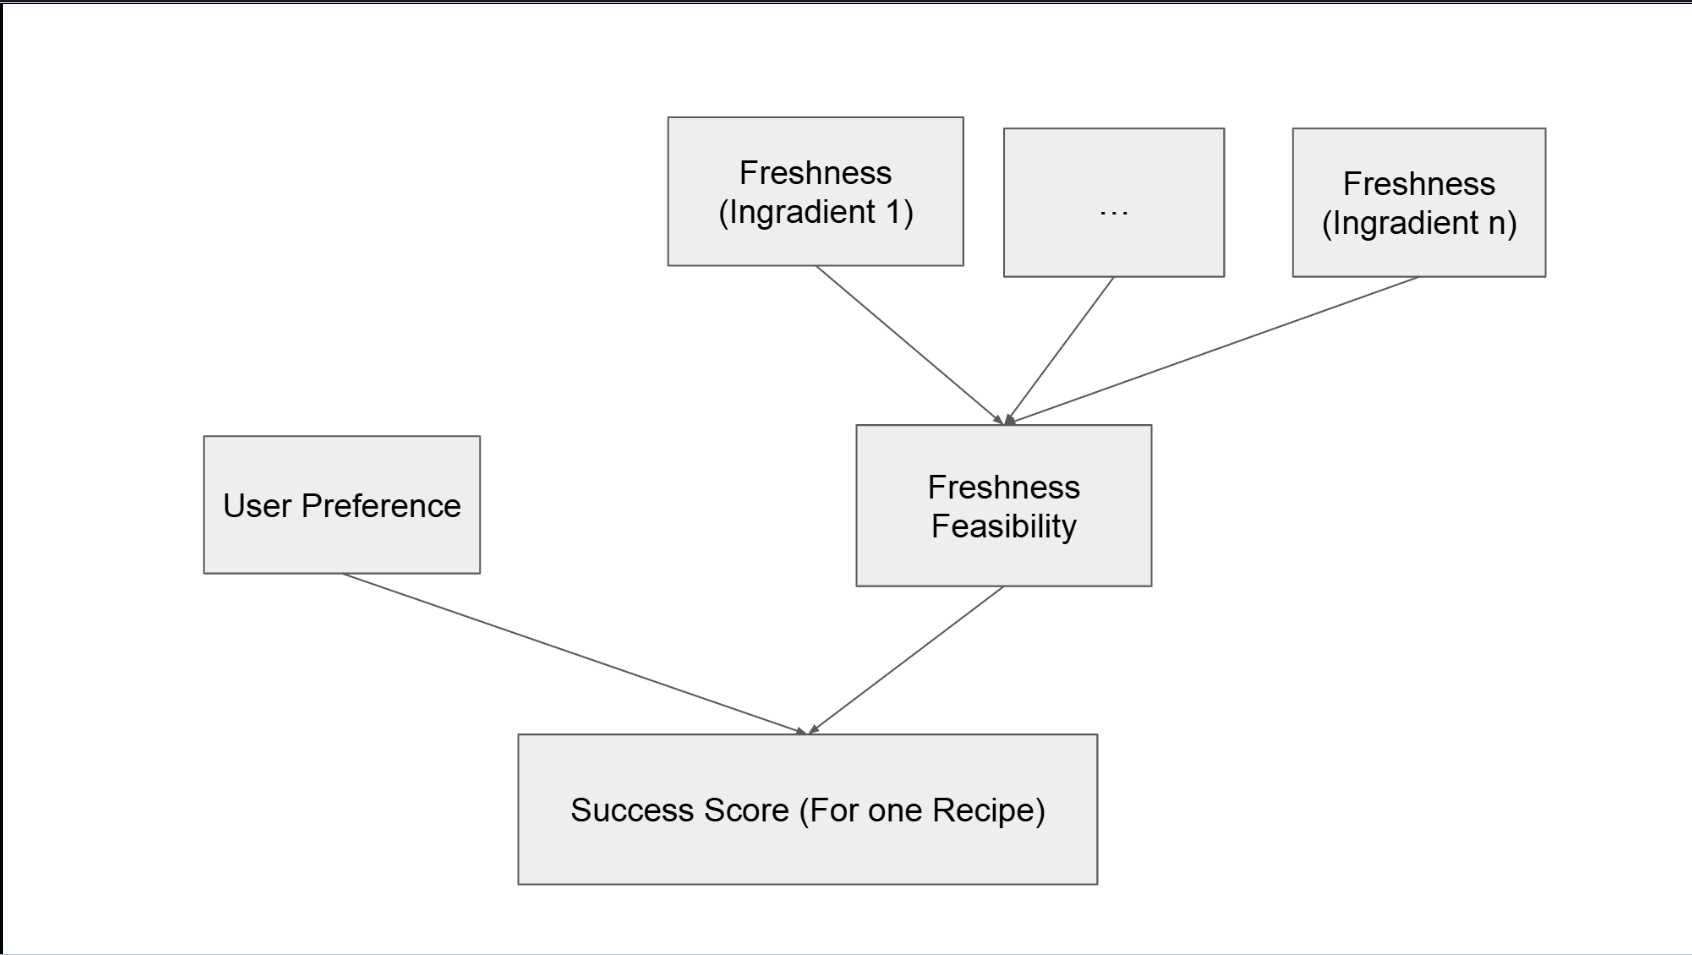
\includegraphics[width=1.0\textwidth]{appendix/Image/BN.png}
    \caption{Bayesian Network structure}
    \label{fig:BN}
\end{figure}

\begin{figure}[ht]
    \centering
    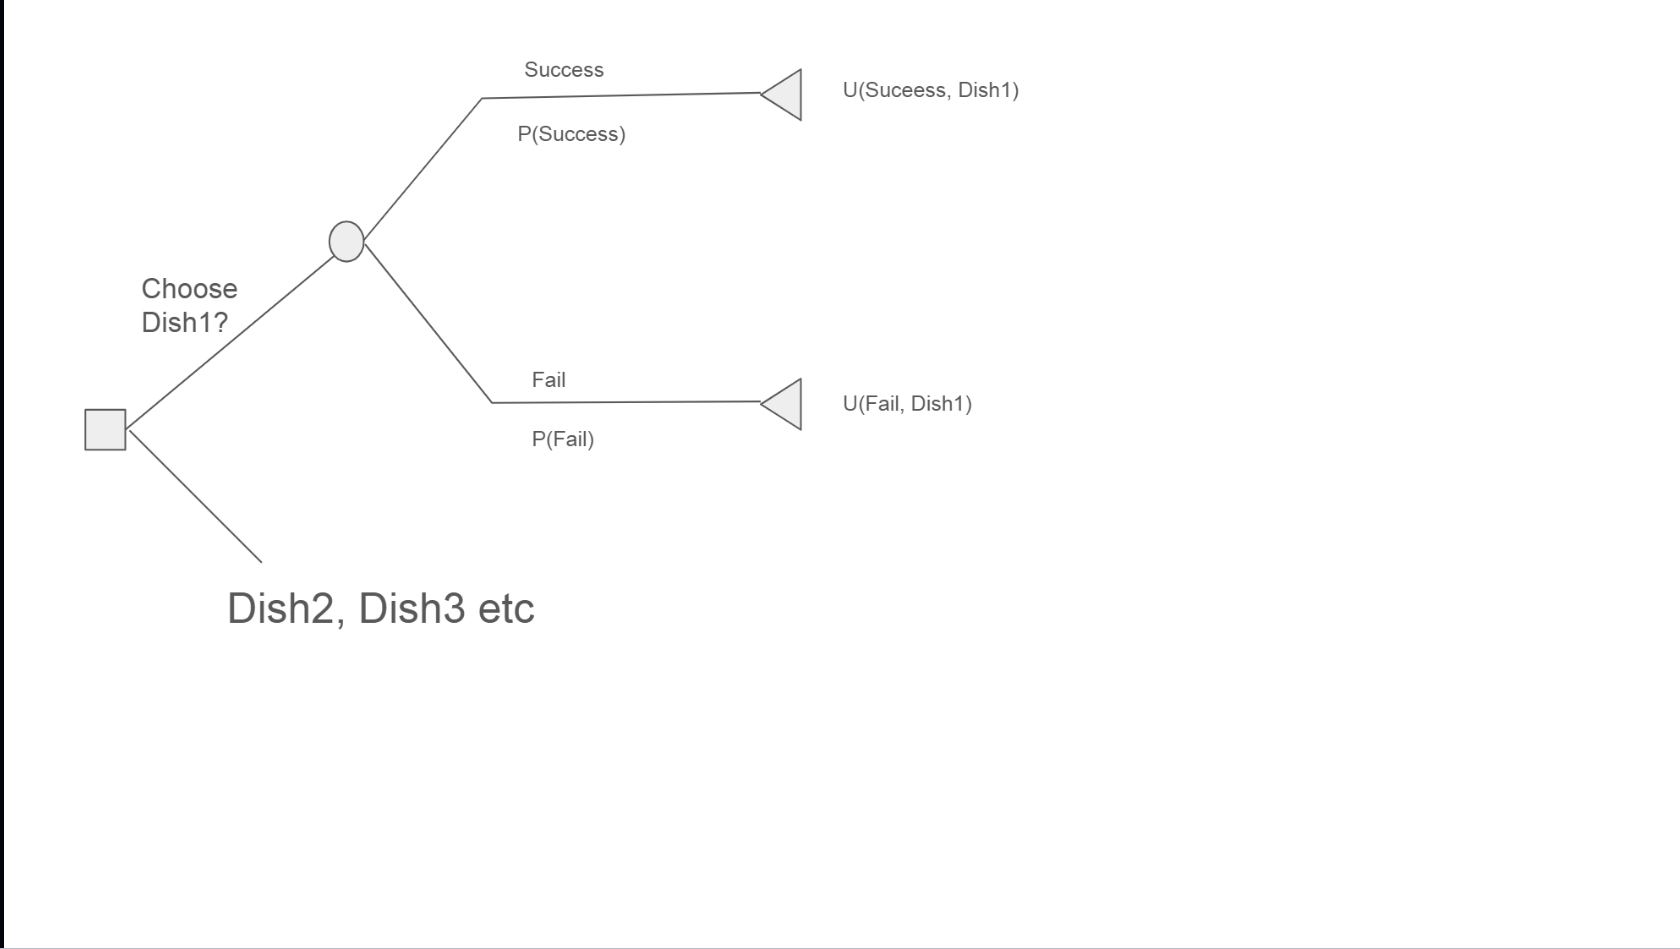
\includegraphics[width=1.0\textwidth]{appendix/Image/Decision-Network.png}
    \caption{Decision Network structure}
    \label{fig:DN}
\end{figure}
\end{appendices}

\bibliographystyle{ACM-Reference-Format}
\bibliography{reference}
%%%%%%%%%%
\end{document}